%%%%%%%%%%%%%%%%%%%%%%%%%%%%%%%%%%%%%
% Slowdown vs Callgrind
%%%%%%%%%%%%%%%%%%%%%%%%%%%%%%%%%%%%%

% Original Table

\iffalse

\begin{table*}[]

\caption{Server: \textbf{comet} - 
 Stat: \textbf{sd} - 
 Tools: pinMain , pinAll , callgrind ,  
 Inputs: B , C ,  
 Nodes: 1 , 4 , 16 , 64 ,  
 Desc: Primary --- This table contains Slowdowns of ParLOT and Callgrind (slowdowns are relative to pure run). The input size is \textbf{B}.  NAS benchmark input sizes are as follows : $size(A) < size(B) < size (C) < size(D) $. I grouped the results of experiments with similar input sizes and nodes (group of 3 rows). Each row is in this format \textbf{Tool.Input.Nodes}. Last column of the table (GM) is GeoMean of all values in that row. By comparing the values of GM row, we can see that ParLOT(both main and all) has better performance comparing to Callgrind. However, it seems that Callgrind scales better}
 
\label{comet_sd_pMpAcg_BC_int_p3.5}\begin{center}
\begin{tabular}{|l|rrrrrrrr|r|}
\hline
                &   bt &   cg &    ep &    ft &   is &   lu &   mg &   sp &   GM \\
\hline
 pinMain.B.1    & 1.55 & 1.82 &  2.68 &  2.11 & 2.48 & 1.31 & 2.57 & 1.33 & 1.91 \\
 pinAll.B.1     & 1.85 & 2.73 &  4.21 &  2.85 & 4.52 & 1.74 & 5.57 & 1.73 & 2.87 \\
 callgrind.B.1  & 8.68 & 6.07 &  9.31 & 10.33 & 2.64 & 7.61 & 3.39 & 6.62 & 6.24 \\
\hline
 pinMain.B.4    & 1.76 & 1.85 &  1.92 &  1.74 & 1.79 & 1.77 & 1.83 & 1.76 & 1.80 \\
 pinAll.B.4     & 2.63 & 3.11 &  3.41 &  2.86 & 3.03 & 2.82 & 3.10 & 2.76 & 2.96 \\
 callgrind.B.4  & 6.13 & 3.63 &  2.95 &  3.50 & 1.46 & 5.41 & 1.43 & 5.98 & 3.34 \\
\hline
 pinMain.B.16   & 2.19 & 2.62 &  2.39 &  1.93 & 1.82 & 2.80 & 2.43 & 2.23 & 2.28 \\
 pinAll.B.16    & 3.73 & 4.20 &  4.36 &  2.96 & 2.84 & 4.30 & 4.49 & 3.71 & 3.77 \\
 callgrind.B.16 & 4.31 & 3.26 &  2.39 &  2.20 & 1.73 & 4.70 & 1.92 & 4.65 & 2.93 \\
\hline
 pinMain.B.64   & 2.45 & 2.72 &  2.45 &  1.99 & 4.34 & 4.56 & 2.31 & 2.46 & 2.79 \\
 pinAll.B.64    & 4.22 & 4.19 &  4.55 &  3.13 & 5.46 & 4.73 & 4.17 & 4.23 & 4.29 \\
 callgrind.B.64 & 2.85 & 2.71 &  1.86 &  2.16 & 4.13 & 4.10 & 1.87 & 3.54 & 2.77 \\
\hline
 pinMain.C.1    & 1.41 & 1.29 &  2.51 &  1.90 & 2.34 & 1.12 & 1.76 & 1.11 & 1.61 \\
 pinAll.C.1     & 1.47 & 1.55 &  3.25 &  2.00 & 3.06 & 1.26 & 2.52 & 1.20 & 1.90 \\
 callgrind.C.1  & 8.52 & 4.51 & 13.47 & 13.13 & 3.81 & 7.93 & 6.31 & 5.15 & 7.13 \\
\hline
 pinMain.C.4    & 1.58 & 1.77 &  2.13 &  1.65 & 1.70 & 1.33 & 1.83 & 1.35 & 1.65 \\
 pinAll.C.4     & 1.93 & 2.52 &  3.35 &  2.24 & 2.65 & 1.77 & 3.09 & 1.71 & 2.34 \\
 callgrind.C.4  & 8.83 & 4.55 &  6.52 &  7.04 & 1.74 & 6.83 & 2.89 & 6.48 & 5.03 \\
\hline
 pinMain.C.16   & 1.82 & 2.39 &  2.47 &  1.52 & 1.83 & 2.22 & 2.40 & 1.82 & 2.03 \\
 pinAll.C.16    & 2.70 & 3.47 &  4.27 &  2.15 & 2.80 & 3.21 & 4.30 & 2.75 & 3.13 \\
 callgrind.C.16 & 6.87 & 4.00 &  3.55 &  2.87 & 1.87 & 6.61 & 2.31 & 6.56 & 3.89 \\
\hline
 pinMain.C.64   & 2.32 & 2.74 &  2.48 &  1.61 & 4.49 & 3.52 & 2.68 & 2.28 & 2.65 \\
 pinAll.C.64    & 3.67 & 4.13 &  4.31 &  2.26 & 5.72 & 4.43 & 4.30 & 3.69 & 3.95 \\
 callgrind.C.64 & 4.37 & 3.49 &  2.20 &  2.52 & 4.25 & 5.52 & 2.13 & 4.70 & 3.45 \\
\hline
\end{tabular}
\end{center}
\end{table*}

\fi



%New Table

\iftrue

\begin{table*}[]

\caption{Server: \textbf{comet} - 
 Stat: \textbf{sd} - 
 Tools: pinMain , pinAll , callgrind ,  
 Inputs: B , C ,  
 Nodes: 1 , 4 , 16 , 64 ,  
 Desc: Primary --- This table contains Slowdowns of ParLOT and Callgrind (slowdowns are relative to pure run). The input size is \textbf{B}.  NAS benchmark input sizes are as follows : $size(A) < size(B) < size (C) < size(D) $. I grouped the results of experiments with similar input sizes and nodes (group of 3 rows). Each row is in this format \textbf{Tool.Input.Nodes}. Last column of the table (GM) is GeoMean of all values in that row. By comparing the values of GM row, we can see that ParLOT(both main and all) has better performance comparing to Callgrind. However, it seems that Callgrind scales better}
 
\label{comet_sd_pMpAcg_BC_int_p3.5}
\begin{center}
\begin{tabular}{|c|c|l|rrrrrrrr|r|}
\hline
\multicolumn{1}{|l|}{Input} & \multicolumn{1}{l|}{\# Nodes} & Tool / App & \multicolumn{1}{c}{bt} & \multicolumn{1}{c}{cg} & \multicolumn{1}{c}{ep} & \multicolumn{1}{c}{ft} & \multicolumn{1}{c}{is} & \multicolumn{1}{c}{lu} & \multicolumn{1}{c}{mg} & \multicolumn{1}{c|}{sp} & \multicolumn{1}{c|}{GM} \\ \hline
\multirow{12}{*}{B} & \multirow{3}{*}{1} & ParLOT(main) & 1.55 & 1.82 & 2.68 & 2.11 & 2.48 & 1.31 & 2.57 & 1.33 & 1.91 \\
 &  & ParLOT(all) & 1.85 & 2.73 & 4.21 & 2.85 & 4.52 & 1.74 & 5.57 & 1.73 & 2.87 \\
 &  & Callgrind & 8.68 & 6.07 & 9.31 & 10.33 & 2.64 & 7.61 & 3.39 & 6.62 & 6.24 \\ \cline{2-12} 
 & \multirow{3}{*}{4} & ParLOT(main) & 1.76 & 1.85 & 1.92 & 1.74 & 1.79 & 1.77 & 1.83 & 1.76 & 1.80 \\
 &  & ParLOT(all) & 2.63 & 3.11 & 3.41 & 2.86 & 3.03 & 2.82 & 3.10 & 2.76 & 2.96 \\
 &  & Callgrind & 6.13 & 3.63 & 2.95 & 3.50 & 1.46 & 5.41 & 1.43 & 5.98 & 3.34 \\ \cline{2-12} 
 & \multirow{3}{*}{16} & ParLOT(main) & 2.19 & 2.62 & 2.39 & 1.93 & 1.82 & 2.80 & 2.43 & 2.23 & 2.28 \\
 &  & ParLOT(all) & 3.73 & 4.20 & 4.36 & 2.96 & 2.84 & 4.30 & 4.49 & 3.71 & 3.77 \\
 &  & Callgrind & 4.31 & 3.26 & 2.39 & 2.20 & 1.73 & 4.70 & 1.92 & 4.65 & 2.93 \\ \cline{2-12} 
 & \multirow{3}{*}{64} & ParLOT(main) & 2.45 & 2.72 & 2.45 & 1.99 & 4.34 & 4.56 & 2.31 & 2.46 & 2.79 \\
 &  & ParLOT(all) & 4.22 & 4.19 & 4.55 & 3.13 & 5.46 & 4.73 & 4.17 & 4.23 & 4.29 \\
 &  & Callgrind & 2.85 & 2.71 & 1.86 & 2.16 & 4.13 & 4.10 & 1.87 & 3.54 & 2.77 \\ \hline
\multirow{12}{*}{C} & \multirow{3}{*}{1} & ParLOT(main) & 1.41 & 1.29 & 2.51 & 1.90 & 2.34 & 1.12 & 1.76 & 1.11 & 1.61 \\
 &  & ParLOT(all) & 1.47 & 1.55 & 3.25 & 2.00 & 3.06 & 1.26 & 2.52 & 1.20 & 1.90 \\
 &  & Callgrind & 8.52 & 4.51 & 13.47 & 13.13 & 3.81 & 7.93 & 6.31 & 5.15 & 7.13 \\ \cline{2-12} 
 & \multirow{3}{*}{4} & ParLOT(main) & 1.58 & 1.77 & 2.13 & 1.65 & 1.70 & 1.33 & 1.83 & 1.35 & 1.65 \\
 &  & ParLOT(all) & 1.93 & 2.52 & 3.35 & 2.24 & 2.65 & 1.77 & 3.09 & 1.71 & 2.34 \\
 &  & Callgrind & 8.83 & 4.55 & 6.52 & 7.04 & 1.74 & 6.83 & 2.89 & 6.48 & 5.03 \\ \cline{2-12} 
 & \multirow{3}{*}{16} & ParLOT(main) & 1.82 & 2.39 & 2.47 & 1.52 & 1.83 & 2.22 & 2.40 & 1.82 & 2.03 \\
 &  & ParLOT(all) & 2.70 & 3.47 & 4.27 & 2.15 & 2.80 & 3.21 & 4.30 & 2.75 & 3.13 \\
 &  & Callgrind & 6.87 & 4.00 & 3.55 & 2.87 & 1.87 & 6.61 & 2.31 & 6.56 & 3.89 \\ \cline{2-12} 
 & \multirow{3}{*}{64} & ParLOT(main) & 2.32 & 2.74 & 2.48 & 1.61 & 4.49 & 3.52 & 2.68 & 2.28 & 2.65 \\
 &  & ParLOT(all) & 3.67 & 4.13 & 4.31 & 2.26 & 5.72 & 4.43 & 4.30 & 3.69 & 3.95 \\
 &  & Callgrind & 4.37 & 3.49 & 2.20 & 2.52 & 4.25 & 5.52 & 2.13 & 4.70 & 3.45 \\ \hline
\end{tabular}
\end{center}
\end{table*}

\fi


\begin{table*}[]
\caption{Server: \textbf{comet} - 
 Stat: \textbf{sd} - 
 Tools: pinMain , pinAll , callgrind ,  
 Inputs: B , C ,  
 Nodes: 1 , 4 , 16 , 64 ,  
 Desc: Primary}
\label{comet_sd_pMpAcg_BC_itn_p3.5}\begin{center}
\begin{tabular}{|l|rrrrrrrr|r|}
\hline
                &   bt &   cg &    ep &    ft &   is &   lu &   mg &   sp &   GM \\
\hline
 pinMain.B.1    & 1.55 & 1.82 &  2.68 &  2.11 & 2.48 & 1.31 & 2.57 & 1.33 & 1.91 \\
 pinMain.B.4    & 1.76 & 1.85 &  1.92 &  1.74 & 1.79 & 1.77 & 1.83 & 1.76 & 1.80 \\
 pinMain.B.16   & 2.19 & 2.62 &  2.39 &  1.93 & 1.82 & 2.80 & 2.43 & 2.23 & 2.28 \\
 pinMain.B.64   & 2.45 & 2.72 &  2.45 &  1.99 & 4.34 & 4.56 & 2.31 & 2.46 & 2.79 \\
 \hline
 AVG            & 1.99 & 2.25 &  2.36 &  1.94 & 2.61 & 2.61 & 2.29 & 1.95 & \textbf{2.20} \\
 \hline
 pinAll.B.1     & 1.85 & 2.73 &  4.21 &  2.85 & 4.52 & 1.74 & 5.57 & 1.73 & 2.87 \\
 pinAll.B.4     & 2.63 & 3.11 &  3.41 &  2.86 & 3.03 & 2.82 & 3.10 & 2.76 & 2.96 \\
 pinAll.B.16    & 3.73 & 4.20 &  4.36 &  2.96 & 2.84 & 4.30 & 4.49 & 3.71 & 3.77 \\
 pinAll.B.64    & 4.22 & 4.19 &  4.55 &  3.13 & 5.46 & 4.73 & 4.17 & 4.23 & 4.29 \\
 \hline
 AVG            & 3.11 & 3.56 &  4.13 &  2.95 & 3.96 & 3.40 & 4.33 & 3.11 & \textbf{3.47} \\
 \hline
 callgrind.B.1  & 8.68 & 6.07 &  9.31 & 10.33 & 2.64 & 7.61 & 3.39 & 6.62 & 6.24 \\
 callgrind.B.4  & 6.13 & 3.63 &  2.95 &  3.50 & 1.46 & 5.41 & 1.43 & 5.98 & 3.34 \\
 callgrind.B.16 & 4.31 & 3.26 &  2.39 &  2.20 & 1.73 & 4.70 & 1.92 & 4.65 & 2.93 \\
 callgrind.B.64 & 2.85 & 2.71 &  1.86 &  2.16 & 4.13 & 4.10 & 1.87 & 3.54 & 2.77 \\
 \hline
 AVG            & 5.49 & 3.92 &  4.13 &  4.55 & 2.49 & 5.46 & 2.15 & 5.20 & \textbf{3.82} \\
 \hline
  \hline
 pinMain.C.1    & 1.41 & 1.29 &  2.51 &  1.90 & 2.34 & 1.12 & 1.76 & 1.11 & 1.61 \\
 pinMain.C.4    & 1.58 & 1.77 &  2.13 &  1.65 & 1.70 & 1.33 & 1.83 & 1.35 & 1.65 \\
 pinMain.C.16   & 1.82 & 2.39 &  2.47 &  1.52 & 1.83 & 2.22 & 2.40 & 1.82 & 2.03 \\
 pinMain.C.64   & 2.32 & 2.74 &  2.48 &  1.61 & 4.49 & 3.52 & 2.68 & 2.28 & 2.65 \\
 \hline
 AVG            & 1.78 & 2.05 &  2.40 &  1.67 & 2.59 & 2.05 & 2.17 & 1.64 & \textbf{1.98} \\
 \hline
 pinAll.C.1     & 1.47 & 1.55 &  3.25 &  2.00 & 3.06 & 1.26 & 2.52 & 1.20 & 1.90 \\
 pinAll.C.4     & 1.93 & 2.52 &  3.35 &  2.24 & 2.65 & 1.77 & 3.09 & 1.71 & 2.34 \\
 pinAll.C.16    & 2.70 & 3.47 &  4.27 &  2.15 & 2.80 & 3.21 & 4.30 & 2.75 & 3.13 \\
 pinAll.C.64    & 3.67 & 4.13 &  4.31 &  2.26 & 5.72 & 4.43 & 4.30 & 3.69 & 3.95 \\
 \hline
 AVG            & 2.44 & 2.92 &  3.79 &  2.16 & 3.56 & 2.67 & 3.55 & 2.34 & \textbf{2.83} \\
 \hline
 callgrind.C.1  & 8.52 & 4.51 & 13.47 & 13.13 & 3.81 & 7.93 & 6.31 & 5.15 & 7.13 \\
 callgrind.C.4  & 8.83 & 4.55 &  6.52 &  7.04 & 1.74 & 6.83 & 2.89 & 6.48 & 5.03 \\
 callgrind.C.16 & 6.87 & 4.00 &  3.55 &  2.87 & 1.87 & 6.61 & 2.31 & 6.56 & 3.89 \\
 callgrind.C.64 & 4.37 & 3.49 &  2.20 &  2.52 & 4.25 & 5.52 & 2.13 & 4.70 & 3.45 \\
 \hline
 AVG            & 7.15 & 4.14 &  6.44 &  6.39 & 2.92 & 6.72 & 3.41 & 5.72 & \textbf{4.88} \\
\hline
\end{tabular}
\end{center}
\end{table*}


Table \ref{comet_sd_pMpAcg_BC_int_p3.5} shows the slowdown of ParLOT (pinMain and pinAll) and Callgrind. It shows slowdowns of same configuration (number of nodes/cores and size of input) next to each other so that we can look into it in more detail.


Table \ref{comet_sd_pMpAcg_BC_itn_p3.5} contains same exact numbers but grouped differently. In big picture, as average, by looking at bold numbers of table \ref{comet_sd_pMpAcg_BC_itn_p3.5}, experiments well shows that ParLOT has better performance on larger input sizes which means longer runs. But for Callgrind it is opposite. For input size B, the average of geomeans of slowdowns is 3.82 and for input C it is 4.88. The key reason of this better performance is more repetition of target data to collect (which is function calls) on larger input sizes, I believe. 

Even when ParLOT gathers system library function calls (pinAll), it has better performance than Callgrind. Figures \ref{comet_chartAvg_sd_B_p3_5} and \ref{comet_chartAvg_sd_C_p3_5} visualizes table \ref{comet_sd_pMpAcg_BC_itn_p3.5} numbers.


\begin{figure*}[!t]
\centering
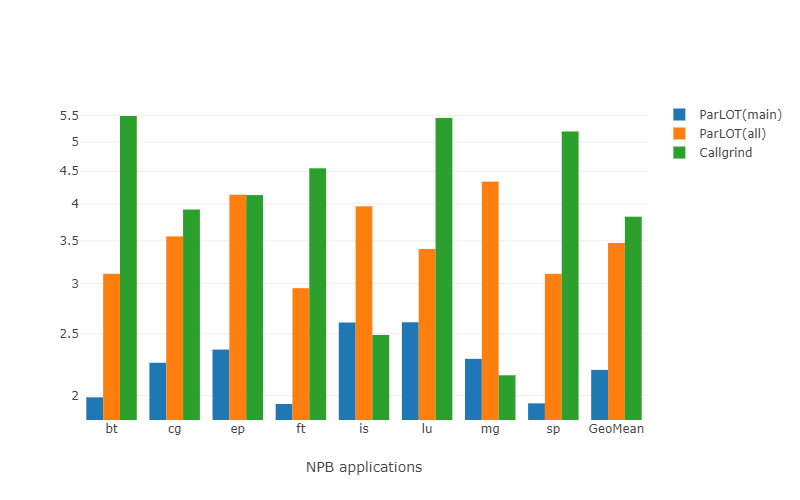
\includegraphics[width=6in]{figs.comet/comet_chartAvg_sd_B_p3_5.png}
\caption{ Input: \textbf{B} - Slowdown of ParLOT(main,all) and Callgrind. Each bar is the average slowdown of each tool on each application for 1, 4 and 16 nodes (16, 64 and 256 cores). Last group of bars is GeoMean (from bold numbers in table \ref{comet_sd_pMpAcg_BC_itn_p3.5}). 
}
\label{comet_chartAvg_sd_B_p3_5}
\end{figure*}


\begin{figure*}[!t]
\centering
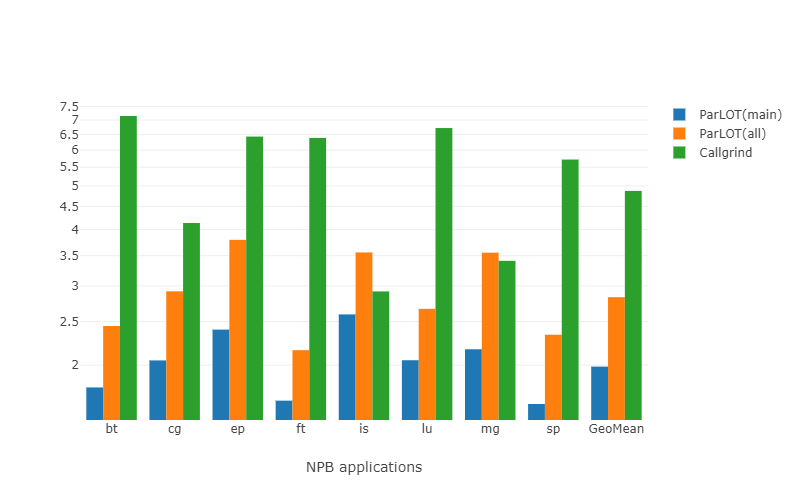
\includegraphics[width=6in]{figs.comet/comet_chartAvg_sd_C_p3_5.png}
\caption{ Input: \textbf{C} - Slowdown of ParLOT(main,all) and Callgrind. Each bar is the average slowdown of each tool on each application for 1, 4 and 16 nodes (16, 64 and 256 cores). Last group of bars is GeoMean (from bold numbers in table \ref{comet_sd_pMpAcg_BC_itn_p3.5}). 
}
\label{comet_chartAvg_sd_C_p3_5}
\end{figure*}


%%%%%%%%%%%%%%%%%%%%%%%%%%%%%%%%%%%%%
% Bandwidth
%%%%%%%%%%%%%%%%%%%%%%%%%%%%%%%%%%%%%

%%%%%%%%%%%%%%%%%%%%%%%
% Compression Ratio
%%%%%%%%%%%%%%%%%%%%%%%


Table \ref{comet_bw_pMpAcg_BC_itn_p3.5} shows the required bandwidth for each tool. In addition to big gap between average slowdown of ParLOT(main) and Callgrind, ParLOT(main) also beats Callgrind in required bandwidth, especially for smaller inputs. Intermediate generated traces by Callgrind are some numbered files contain pure ascii text. There is no compression involved (one of Callgrind options which can be enabled or disabled is compressing/encoding only the name of function calls which was enabled on these experiments by default). Each Callgrind trace file contains a sequence of function names (or their code) and a few other numbers for each function showing the parent callers. [ there is a tool callgrind\_ annotate which displays different reports from the generated traces. After I check all possible options, I add more analysis here. But according to table \ref{comet_cr_pMpA_BC_itn_p3.5}, for example for ParLOT(all) where the average compression ratio for input C is 644.38, and the correspondent required bandwidth which is 56.38, it shows that ParLOT can collect almost 36 MB worth of data per core per second where it only needs 56.38 KB/S bandwidth.] \\


\begin{table*}[]
\caption{Server: \textbf{comet} - 
 Stat: \textbf{bw} - 
 Tools: pinMain , pinAll , callgrind ,  
 Inputs: B , C ,  
 Nodes: 1 , 4 , 16 , 64 ,  
 Desc: Primary
This table is showing the required bandwidth for each application (KiloBytes per core per second). $ReqBW_x = TraceSize_x (KB) / (\# of cores)_x / Runtime_x (S)$
. Clearly ParLOT(main) is beating Callgrind while they both generate the same information. ParLOT(all) bandwidth is the highest but with capturing all of the function calls within a single execution, there is no surprise. Figures \ref{comet_chartAvg_bw_B_p3_5} and \ref{comet_chartAvg_bw_C_p3_5} visualize these numbers (Average values) 
 }
\label{comet_bw_pMpAcg_BC_itn_p3.5}\begin{center}
\begin{tabular}{|l|rrrrrrrr|r|}
\hline
                &    bt &     cg &    ep &    ft &    is &     lu &    mg &     sp &    GM \\
\hline
 pinMain.B.1    &  4.72 &  21.86 &  3.83 &  1.52 &  0.79 &   2.39 &  5.62 &   5.36 &  3.69 \\
 pinMain.B.4    & 14.28 &  41.08 &  1.89 &  3.48 &  2.24 &  21.48 &  6.45 &  15.85 &  8.12 \\
 pinMain.B.16   & 14.31 &  46.59 &  1.45 &  4.86 &  3.40 &  31.79 &  6.53 &  18.55 &  9.41 \\
 pinMain.B.64   & 18.56 &  43.59 &  1.25 &  4.56 &  4.49 &  27.07 &  5.63 &  29.62 &  9.92 \\
 \hline
 AVG            & 12.97 &  38.28 &  2.10 &  3.60 &  2.73 &  20.68 &  6.06 &  17.35 &  \textbf{7.79} \\
 \hline
 pinAll.B.1     & 48.71 &  89.39 & 47.23 & 45.63 & 59.98 &  53.62 & 60.81 &  54.33 & 56.21 \\
 pinAll.B.4     & 61.84 & 101.23 & 45.21 & 55.12 & 53.20 &  71.09 & 54.85 &  73.62 & 62.68 \\
 pinAll.B.16    & 73.95 & 116.87 & 47.37 & 48.88 & 47.79 & 100.91 & 55.80 &  84.61 & 67.97 \\
 pinAll.B.64    & 81.80 & 110.15 & 44.16 & 47.98 & 37.84 & 100.26 & 52.67 &  99.90 & 66.47 \\
 \hline
 AVG            & 66.58 & 104.41 & 45.99 & 49.40 & 49.70 &  81.47 & 56.03 &  78.12 & \textbf{63.33} \\
 \hline
 callgrind.B.1  &  1.57 &   7.69 &  7.39 &  4.56 & 39.49 &   2.61 & 34.41 &   2.71 &  6.67 \\
 callgrind.B.4  &  6.51 &  16.01 & 22.10 & 15.65 & 45.46 &   8.63 & 45.47 &   7.78 & 16.31 \\
 callgrind.B.16 & 17.20 &  24.62 & 37.42 & 23.84 & 29.87 &  16.23 & 51.49 &  15.81 & 24.93 \\
 callgrind.B.64 & 26.82 &  27.65 & 45.93 & 25.14 & 11.04 &  17.75 & 45.27 &  20.20 & 25.02 \\
 \hline
 AVG            & 13.03 &  18.99 & 28.21 & 17.30 & 31.47 &  11.30 & 44.16 &  11.62 & \textbf{18.23} \\
 \hline
 \hline
 pinMain.C.1    &  1.82 &  16.96 &  5.15 &  1.16 &  0.69 &   0.77 &  3.56 &   1.40 &  2.17 \\
 pinMain.C.4    &  7.53 &  44.87 &  3.00 &  2.50 &  2.12 &  20.13 &  7.08 &  13.74 &  7.55 \\
 pinMain.C.16   & 16.30 &  55.04 &  1.84 &  6.10 &  3.35 &  34.09 &  7.24 &  20.68 & 10.70 \\
 pinMain.C.64   & 17.45 &  61.43 &  1.30 &  5.93 &  4.42 &  38.28 &  5.62 &  26.09 & 10.94 \\
 \hline
 AVG            & 10.77 &  44.58 &  2.82 &  3.92 &  2.65 &  23.32 &  5.88 &  15.48 &  \textbf{7.84} \\
 \hline
 pinAll.C.1     & 17.80 &  53.37 & 26.34 & 20.89 & 48.31 &  25.31 & 52.61 &  19.46 & 29.99 \\
 pinAll.C.4     & 51.78 &  95.84 & 36.80 & 43.82 & 51.40 &  58.39 & 54.18 &  65.77 & 55.15 \\
 pinAll.C.16    & 75.38 & 121.03 & 44.29 & 61.39 & 46.90 & 101.05 & 56.49 & 101.32 & 71.37 \\
 pinAll.C.64    & 80.63 & 135.19 & 43.49 & 46.28 & 37.09 & 117.87 & 54.05 &  99.02 & 68.99 \\
 \hline
 AVG            & 56.40 & 101.36 & 37.73 & 43.09 & 45.93 &  75.66 & 54.33 &  71.39 & \textbf{56.38} \\
 \hline
 callgrind.C.1  &  0.40 &   3.09 &  1.96 &  1.05 & 14.60 &   0.70 &  6.96 &   0.75 &  1.85 \\
 callgrind.C.4  &  1.78 &   8.87 &  7.74 &  4.48 & 31.74 &   2.82 & 21.03 &   2.78 &  6.41 \\
 callgrind.C.16 &  6.01 &  15.82 & 22.86 & 10.75 & 26.50 &   7.45 & 39.05 &   6.96 & 13.72 \\
 callgrind.C.64 & 14.32 &  19.56 & 35.75 & 12.17 & 11.07 &  11.86 & 40.69 &  12.83 & 17.39 \\
 \hline
 AVG            &  5.63 &  11.84 & 17.08 &  7.11 & 20.98 &   5.71 & 26.93 &   5.83 &  \textbf{9.84} \\
\hline
\end{tabular}
\end{center}
\end{table*}


\begin{figure*}[!t]
\centering
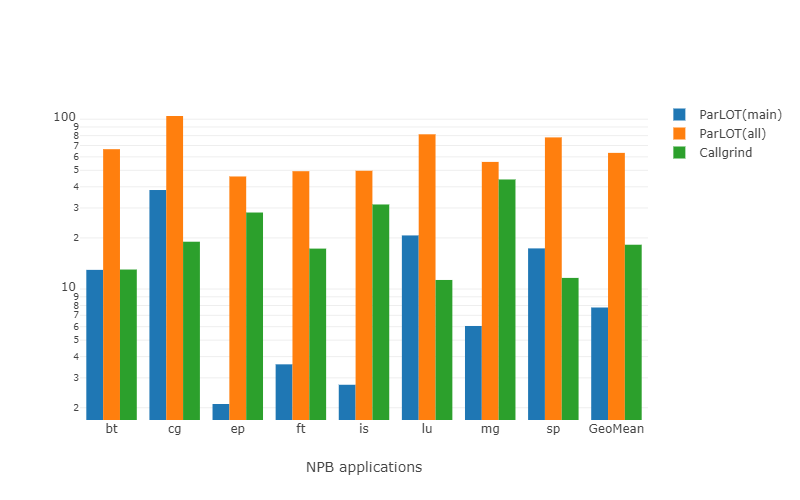
\includegraphics[width=6in]{figs.comet/comet_chartAvg_bw_B_p3_5.png}
\caption{ Input: \textbf{B} - Required Bandwidth per core (KB/s)
}
\label{comet_chartAvg_bw_B_p3_5}
\end{figure*}

\begin{figure*}[!t]
\centering
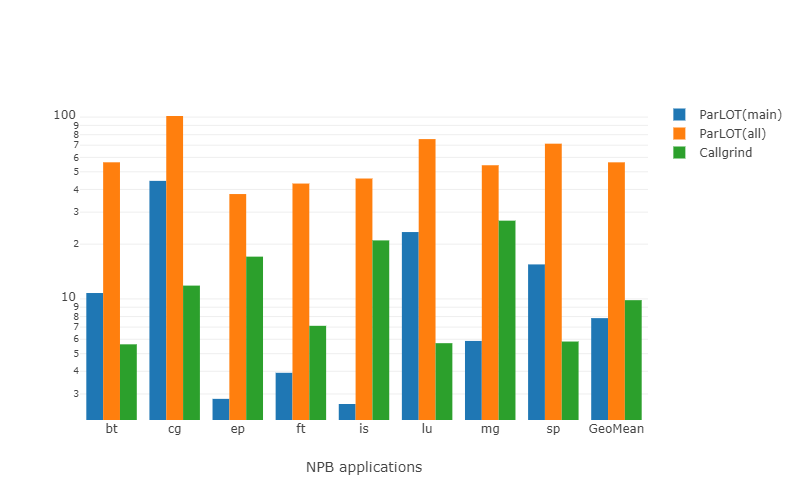
\includegraphics[width=6in]{figs.comet/comet_chartAvg_bw_C_p3_5.png}
\caption{ Input: \textbf{C}  - Required Bandwidth per core (KB/s)
}
\label{comet_chartAvg_bw_C_p3_5}
\end{figure*}



%%%%%%%%%%%%%%%%%%%%%%%
% Detail runtimes
%%%%%%%%%%%%%%%%%%%%%%%

\begin{table*}[]
\caption{Server: \textbf{comet} - 
 Stat: \textbf{cr} - 
 Tools: pinMain , pinAll ,  
 Inputs: B , C ,  
 Nodes: 1 , 4 , 16 , 64 ,  
 Desc: Primary}
\label{comet_cr_pMpA_BC_itn_p3.5}\begin{center}
\begin{tabular}{|l|rrrrrrrr|r|}
\hline
              &      bt &     cg &       ep &       ft &       is &     lu &     mg &      sp &      GM \\
\hline
 pinMain.B.1  & 3035.93 &  94.35 & 12456.18 & 12173.49 &  9718.38 & 167.72 &  99.08 &  878.27 & 1255.17 \\
 pinMain.B.4  &  586.64 &  82.48 & 10368.41 &  1737.09 &   909.20 & 140.29 & 254.95 &  338.16 &  559.36 \\
 pinMain.B.16 &  346.66 & 113.28 &  8563.85 &  1077.35 &  1200.57 & 178.98 & 387.63 &  123.02 &  496.83 \\
 pinMain.B.64 &  252.24 & 147.78 &  7611.04 &  1122.62 &  1907.95 & 366.80 & 437.31 &  152.91 &  591.11 \\
 \hline
 AVG          & 1055.37 & 109.47 &  9749.87 &  4027.64 &  3434.03 & 213.45 & 294.74 &  373.09 &  \textbf{725.62} \\
 \hline
 pinAll.B.1   &  514.51 & 137.41 &  3335.77 &  1226.74 &   543.18 & 314.63 & 260.87 &  303.88 &  500.21 \\
 pinAll.B.4   &  315.71 & 137.21 &  1266.92 &   436.15 &   316.16 & 287.25 & 329.57 &  199.66 &  330.70 \\
 pinAll.B.16  &  226.86 & 181.58 &  1246.66 &  1026.53 &   927.09 & 299.30 & 469.29 &  171.52 &  430.39 \\
 pinAll.B.64  &  329.23 & 247.30 &  1394.07 &  1043.94 &  1984.62 & 410.32 & 548.47 &  307.16 &  597.55 \\
 \hline
 AVG          &  346.58 & 175.88 &  1810.86 &   933.34 &   942.76 & 327.88 & 402.05 &  245.56 &  \textbf{464.71} \\
 \hline
 \hline
 pinMain.C.1  & 8618.95 & 111.16 & 13067.96 & 21335.57 & 21856.49 & 350.03 & 247.44 & 1977.43 & 2371.35 \\
 pinMain.C.4  & 1910.64 & 110.45 & 12418.66 &  6520.34 &  2256.56 & 112.77 & 267.98 &  472.68 &  928.16 \\
 pinMain.C.16 &  580.79 & 133.24 & 11017.36 &  1239.31 &  1347.88 & 164.47 & 396.86 &  143.13 &  582.78 \\
 pinMain.C.64 &  322.83 & 131.92 &  9154.99 &  1065.12 &  1896.25 & 223.69 & 465.74 &  168.89 &  585.74 \\
 \hline
 AVG          & 2858.30 & 121.69 & 11414.74 &  7540.09 &  6839.30 & 212.74 & 344.50 &  690.53 & \textbf{1117.01} \\
 \hline
 pinAll.C.1   & 2579.37 & 181.76 &  7376.96 &  5143.08 &  1520.42 & 408.21 & 314.77 &  650.73 & 1107.37 \\
 pinAll.C.4   &  448.61 & 161.32 &  3194.58 &  1062.94 &   527.34 & 274.70 & 319.35 &  237.43 &  477.42 \\
 pinAll.C.16  &  285.05 & 185.74 &  1765.49 &   588.86 &  1106.34 & 273.63 & 467.35 &  141.69 &  426.92 \\
 pinAll.C.64  &  290.00 & 214.68 &  1512.89 &  1237.30 &  2038.72 & 329.04 & 496.21 &  270.83 &  565.82 \\
 \hline
 AVG          &  900.76 & 185.88 &  3462.48 &  2008.05 &  1298.21 & 321.39 & 399.42 &  325.17 &  \textbf{644.38} \\
\hline
\end{tabular}
\end{center}
\end{table*}




\begin{table*}[]
\caption{Server: \textbf{comet} - 
 Stat: \textbf{sd} - 
 Tools:  
 Inputs: B ,  
 Nodes: 1 , 4 , 16 , 64 ,  
 Desc: Detail Report}
\begin{center}
\label{comet_wo_det_Main_all_B_p3.5}
\scalebox{0.95}{
\begin{tabular}{|c|c|rrr|rrr|rrr|rrr|} 
\hline 
\multicolumn{1}{|l|}{\multirow{2}{*}{\textbf{Input: B}}} & \multicolumn{1}{r|}{Nodes :}    & \multicolumn{3}{c|}{1}  & \multicolumn{3}{c|}{4} & \multicolumn{3}{c|}{16}  & \multicolumn{3}{c|}{64} \\ \cline{2-14} 
\multicolumn{1}{|l|}{} & \multicolumn{1}{r|}{Detail Tools:} & \multicolumn{1}{c}{npin} & \multicolumn{1}{c}{ParLOT} & \multicolumn{1}{c|}{wpin} & \multicolumn{1}{c}{npin} & \multicolumn{1}{c}{ParLOT} & \multicolumn{1}{c|}{wpin} & \multicolumn{1}{c}{npin} & \multicolumn{1}{c}{ParLOT} & \multicolumn{1}{c|}{wpin} & \multicolumn{1}{c}{npin} & \multicolumn{1}{c}{ParLOT} & \multicolumn{1}{c|}{wpin} \\
\hline
\multirow{9}{*}{Main} &  bt  &  1.50  &  1.55  &   5.66  &  1.74  &  1.76  &  5.19  &  2.21  & \cellcolor{blue!25} 2.19  &  5.98  &  2.29  &  2.45  &  5.42 \\
 &  cg  &  1.75  &  1.82  &   2.39  &  1.95  & \cellcolor{blue!25} 1.85  &  2.64  &  2.72  & \cellcolor{blue!25} 2.62  &  5.06  &  2.67  &  2.72  &  7.01 \\
 &  ep  &  2.97  & \cellcolor{blue!25} 2.68  &  21.44  &  2.07  & \cellcolor{blue!25} 1.92  &  5.82  &  2.58  & \cellcolor{blue!25} 2.39  &  3.76  &  2.81  & \cellcolor{blue!25} 2.45  &  2.85 \\
 &  ft  &  1.87  &  2.11  &   6.29  &  1.76  & \cellcolor{blue!25} 1.74  &  2.85  &  2.13  & \cellcolor{blue!25} 1.93  &  2.25  &  2.23  & \cellcolor{blue!25} 1.99  &  2.22 \\
 &  is  &  2.51  & \cellcolor{blue!25} 2.48  &   4.87  &  1.80  & \cellcolor{blue!25} 1.79  &  2.08  &  2.11  & \cellcolor{blue!25} 1.82  &  1.90  &  4.76  & \cellcolor{blue!25} 4.34  &  5.75 \\
 &  lu  &  1.32  & \cellcolor{blue!25} 1.31  &   1.44  &  1.77  &  1.77  &  2.27  &  2.74  &  2.80  &  3.63  &  3.05  &  4.56  &  6.64 \\
 &  mg  &  2.64  & \cellcolor{blue!25} 2.57  &   2.80  &  1.75  &  1.83  &  1.79  &  2.64  & \cellcolor{blue!25} 2.43  &  2.73  &  2.37  & \cellcolor{blue!25} 2.31  &  2.49 \\
 &  sp  &  1.35  & \cellcolor{blue!25} 1.33  &   2.47  &  1.74  &  1.76  &  3.72  &  2.15  &  2.23  &  2.52  &  2.29  &  2.46  &  3.65 \\
 &  GM  &  1.90  &  1.91  &   4.15  &  1.82  & \cellcolor{blue!25} 1.80  &  3.03  &  2.40  & \cellcolor{blue!25} 2.28  &  3.24  &  2.72  &  2.79  &  4.12 \\
\hline 
\end{tabular} }

\end{center}
\end{table*}


\begin{table*}[]
\caption{Server: \textbf{comet} - 
 Stat: \textbf{sd} - 
 Tools:  
 Inputs: B ,  
 Nodes: 1 , 4 , 16 , 64 ,  
 Desc: Detail Report}
\begin{center}
\label{comet_wo_det_All_all_B_p3.5}
\scalebox{0.95}{
\begin{tabular}{|c|c|rrr|rrr|rrr|rrr|} 
\hline 
\multicolumn{1}{|l|}{\multirow{2}{*}{\textbf{Input: B}}} & \multicolumn{1}{r|}{Nodes :}    & \multicolumn{3}{c|}{1}  & \multicolumn{3}{c|}{4} & \multicolumn{3}{c|}{16}  & \multicolumn{3}{c|}{64} \\ \cline{2-14} 
\multicolumn{1}{|l|}{} & \multicolumn{1}{r|}{Detail Tools:} & \multicolumn{1}{c}{npin} & \multicolumn{1}{c}{ParLOT} & \multicolumn{1}{c|}{wpin} & \multicolumn{1}{c}{npin} & \multicolumn{1}{c}{ParLOT} & \multicolumn{1}{c|}{wpin} & \multicolumn{1}{c}{npin} & \multicolumn{1}{c}{ParLOT} & \multicolumn{1}{c|}{wpin} & \multicolumn{1}{c}{npin} & \multicolumn{1}{c}{ParLOT} & \multicolumn{1}{c|}{wpin} \\
\hline
\multirow{9}{*}{All} &  bt  &  1.76  &  1.85  &   6.23  &  2.39  &  2.63  &  6.39  &  3.40  &  3.73  &  10.64  &  3.74  &  4.22  &   9.47 \\
 &  cg  &  2.72  &  2.73  &   3.80  &  2.88  &  3.11  &  4.64  &  4.08  &  4.20  &  16.45  &  4.10  &  4.19  &  14.32 \\
 &  ep  &  4.42  & \cellcolor{blue!25} 4.21  &  23.24  &  3.25  &  3.41  &  7.16  &  4.27  &  4.36  &   5.67  &  4.43  &  4.55  &   5.13 \\
 &  ft  &  2.82  &  2.85  &   6.98  &  2.65  &  2.86  &  3.85  &  2.96  &  2.96  &   4.66  &  3.60  & \cellcolor{blue!25} 3.13  &   3.91 \\
 &  is  &  4.67  & \cellcolor{blue!25} 4.52  &   7.14  &  2.89  &  3.03  &  3.45  &  3.02  & \cellcolor{blue!25} 2.84  &   3.46  &  5.43  &  5.46  &  11.41 \\
 &  lu  &  1.71  &  1.74  &   2.41  &  2.54  &  2.82  &  4.91  &  4.09  &  4.30  &  11.60  &  4.48  &  4.73  &  25.53 \\
 &  mg  &  4.93  &  5.57  &   5.66  &  2.80  &  3.10  &  3.17  &  4.35  &  4.49  &   5.34  &  3.98  &  4.17  &   5.31 \\
 &  sp  &  1.70  &  1.73  &   3.13  &  2.54  &  2.76  &  5.32  &  3.43  &  3.71  &   7.39  &  3.66  &  4.23  &  22.13 \\
 &  GM  &  2.82  &  2.87  &   5.74  &  2.73  &  2.96  &  4.69  &  3.66  &  3.77  &   7.21  &  4.14  &  4.29  &   9.91 \\
\hline 
\end{tabular} }

\end{center}
\end{table*}



\begin{table*}[]
\caption{Server: \textbf{comet} - 
 Stat: \textbf{sd} - 
 Tools:  
 Inputs: C ,  
 Nodes: 1 , 4 , 16 , 64 ,  
 Desc: Detail Report}
\begin{center}
\label{comet_wo_det_Main_all_C_p3.5}
\scalebox{0.95}{
\begin{tabular}{|c|c|rrr|rrr|rrr|rrr|} 
\hline 
\multicolumn{1}{|l|}{\multirow{2}{*}{\textbf{Input: C}}} & \multicolumn{1}{r|}{Nodes :}    & \multicolumn{3}{c|}{1}  & \multicolumn{3}{c|}{4} & \multicolumn{3}{c|}{16}  & \multicolumn{3}{c|}{64} \\ \cline{2-14} 
\multicolumn{1}{|l|}{} & \multicolumn{1}{r|}{Detail Tools:} & \multicolumn{1}{c}{npin} & \multicolumn{1}{c}{ParLOT} & \multicolumn{1}{c|}{wpin} & \multicolumn{1}{c}{npin} & \multicolumn{1}{c}{ParLOT} & \multicolumn{1}{c|}{wpin} & \multicolumn{1}{c}{npin} & \multicolumn{1}{c}{ParLOT} & \multicolumn{1}{c|}{wpin} & \multicolumn{1}{c}{npin} & \multicolumn{1}{c}{ParLOT} & \multicolumn{1}{c|}{wpin} \\
\hline
\multirow{9}{*}{Main} &  bt  &  1.36  &  1.41  &   5.36  &  1.53  &  1.58  &   5.86  &  2.09  & \cellcolor{blue!25} 1.82  &   6.05  &  2.10  &  2.32  &   5.76 \\
 &  cg  &  1.27  &  1.29  &   1.75  &  1.68  &  1.77  &   3.02  &  2.82  & \cellcolor{blue!25} 2.39  &   6.19  &  2.83  & \cellcolor{blue!25} 2.74  &  15.57 \\
 &  ep  &  2.95  & \cellcolor{blue!25} 2.51  &  30.50  &  2.27  & \cellcolor{blue!25} 2.13  &  14.23  &  2.83  & \cellcolor{blue!25} 2.47  &  10.32  &  2.58  & \cellcolor{blue!25} 2.48  &   3.84 \\
 &  ft  &  1.50  &  1.90  &   9.21  &  1.56  &  1.65  &   5.23  &  1.70  & \cellcolor{blue!25} 1.52  &   3.27  &  1.75  & \cellcolor{blue!25} 1.61  &   2.23 \\
 &  is  &  2.26  &  2.34  &   7.28  &  1.72  & \cellcolor{blue!25} 1.70  &   2.75  &  2.05  & \cellcolor{blue!25} 1.83  &   2.34  &  4.73  & \cellcolor{blue!25} 4.49  &   6.66 \\
 &  lu  &  1.12  &  1.12  &   1.19  &  1.32  &  1.33  &   1.59  &  2.16  &  2.22  &   3.95  &  2.95  &  3.52  &   9.77 \\
 &  mg  &  1.75  &  1.76  &   2.02  &  1.84  & \cellcolor{blue!25} 1.83  &   2.03  &  2.47  & \cellcolor{blue!25} 2.40  &   2.86  &  2.47  &  2.68  &   3.28 \\
 &  sp  &  1.10  &  1.11  &   1.63  &  1.36  & \cellcolor{blue!25} 1.35  &   2.88  &  1.78  &  1.82  &   2.38  &  2.11  &  2.28  &   5.58 \\
 &  GM  &  1.57  &  1.61  &   4.07  &  1.64  &  1.65  &   3.68  &  2.20  & \cellcolor{blue!25} 2.03  &   4.10  &  2.58  &  2.65  &   5.56 \\
\hline 
\end{tabular} }

\end{center}
\end{table*}


\begin{table*}[]
\caption{Server: \textbf{comet} - 
 Stat: \textbf{sd} - 
 Tools:  
 Inputs: C ,  
 Nodes: 1 , 4 , 16 , 64 ,  
 Desc: Detail Report}
\begin{center}
\label{comet_wo_det_All_all_C_p3.5}
\scalebox{0.95}{
\begin{tabular}{|c|c|rrr|rrr|rrr|rrr|} 
\hline 
\multicolumn{1}{|l|}{\multirow{2}{*}{\textbf{Input: C}}} & \multicolumn{1}{r|}{Nodes :}    & \multicolumn{3}{c|}{1}  & \multicolumn{3}{c|}{4} & \multicolumn{3}{c|}{16}  & \multicolumn{3}{c|}{64} \\ \cline{2-14} 
\multicolumn{1}{|l|}{} & \multicolumn{1}{r|}{Detail Tools:} & \multicolumn{1}{c}{npin} & \multicolumn{1}{c}{ParLOT} & \multicolumn{1}{c|}{wpin} & \multicolumn{1}{c}{npin} & \multicolumn{1}{c}{ParLOT} & \multicolumn{1}{c|}{wpin} & \multicolumn{1}{c}{npin} & \multicolumn{1}{c}{ParLOT} & \multicolumn{1}{c|}{wpin} & \multicolumn{1}{c}{npin} & \multicolumn{1}{c}{ParLOT} & \multicolumn{1}{c|}{wpin} \\
\hline
\multirow{9}{*}{All} &  bt  &  1.43  &  1.47  &   5.31  &  1.79  &  1.93  &   6.32  &  2.51  &  2.70  &   8.84  &  3.20  &  3.67  &   9.67 \\
 &  cg  &  1.57  & \cellcolor{blue!25} 1.55  &   2.08  &  2.44  &  2.52  &   4.35  &  3.74  & \cellcolor{blue!25} 3.47  &  11.74  &  4.13  &  4.13  &  17.15 \\
 &  ep  &  3.56  & \cellcolor{blue!25} 3.25  &  30.05  &  3.16  &  3.35  &  14.92  &  4.15  &  4.27  &   9.10  &  4.25  &  4.31  &   5.40 \\
 &  ft  &  1.78  &  2.00  &   9.55  &  2.15  &  2.24  &   5.60  &  2.09  &  2.15  &   4.40  &  2.29  & \cellcolor{blue!25} 2.26  &   3.35 \\
 &  is  &  3.35  & \cellcolor{blue!25} 3.06  &   8.20  &  2.65  &  2.65  &   3.86  &  2.95  & \cellcolor{blue!25} 2.80  &   3.53  &  5.59  &  5.72  &   8.98 \\
 &  lu  &  1.23  &  1.26  &   1.52  &  1.70  &  1.77  &   2.94  &  3.09  &  3.21  &   8.28  &  4.22  &  4.43  &  19.13 \\
 &  mg  &  2.67  & \cellcolor{blue!25} 2.52  &   2.96  &  2.92  &  3.09  &   3.32  &  4.04  &  4.30  &   4.81  &  4.04  &  4.30  &   5.25 \\
 &  sp  &  1.17  &  1.20  &   1.67  &  1.65  &  1.71  &   3.57  &  2.56  &  2.75  &   5.38  &  3.16  &  3.69  &  10.48 \\
 &  GM  &  1.92  & \cellcolor{blue!25} 1.90  &   4.58  &  2.24  &  2.34  &   4.86  &  3.06  &  3.13  &   6.49  &  3.75  &  3.95  &   8.54 \\
\hline 
\end{tabular} }

\end{center}
\end{table*}





\begin{table*}[]
\caption{Server: \textbf{comet} - 
 Stat: \textbf{sd} - 
 Tools:  
 Inputs: B ,  
 Nodes: 1 , 4 , 16 , 64 ,  
 Desc: Detail Report}
\begin{center}
\label{comet_wa_det_Main_all_B_p3.5}
\scalebox{0.95}{
\begin{tabular}{|c|c|rrrr|rrrr|rrrr|rrrr|} 
\hline 
\multicolumn{1}{|l|}{\multirow{2}{*}{\textbf{Input: B}}} & \multicolumn{1}{r|}{Nodes :}    & \multicolumn{4}{c|}{1}  & \multicolumn{4}{c|}{4} & \multicolumn{4}{c|}{16}  & \multicolumn{4}{c|}{64} \\ \cline{2-18} 
\multicolumn{1}{|l|}{} & \multicolumn{1}{r|}{Detail Tools:} & \multicolumn{1}{c}{npin} & \multicolumn{1}{c}{apin} & \multicolumn{1}{c}{ParLOT} & \multicolumn{1}{c|}{wpin} & \multicolumn{1}{c}{npin} & \multicolumn{1}{c}{apin} & \multicolumn{1}{c}{ParLOT} & \multicolumn{1}{c|}{wpin} & \multicolumn{1}{c}{npin} & \multicolumn{1}{c}{apin} & \multicolumn{1}{c}{ParLOT} & \multicolumn{1}{c|}{wpin} & \multicolumn{1}{c}{npin} & \multicolumn{1}{c}{apin} & \multicolumn{1}{c}{ParLOT} & \multicolumn{1}{c|}{wpin} \\
\hline
\multirow{9}{*}{Main} &  bt  &  1.50  &  1.56  & \cellcolor{blue!25} 1.55  &   5.66  &  1.74  &  1.78  & \cellcolor{blue!25} 1.76  &  5.19  &  2.21  &  2.25  & \cellcolor{blue!25} 2.19  &  5.98  &  2.29  &  2.50  & \cellcolor{blue!25} 2.45  &  5.42 \\
 &  cg  &  1.75  &  1.81  &  1.82  &   2.39  &  1.95  & \cellcolor{blue!25} 1.84  &  1.85  &  2.64  &  2.72  &  2.72  & \cellcolor{blue!25} 2.62  &  5.06  &  2.67  & \cellcolor{blue!25} 2.53  &  2.72  &  7.01 \\
 &  ep  &  2.97  & \cellcolor{blue!25} 2.69  & \cellcolor{blue!25} 2.68  &  21.44  &  2.07  & \cellcolor{blue!25} 1.91  &  1.92  &  5.82  &  2.58  & \cellcolor{blue!25} 2.38  &  2.39  &  3.76  &  2.81  & \cellcolor{blue!25} 2.50  & \cellcolor{blue!25} 2.45  &  2.85 \\
 &  ft  &  1.87  &  2.11  &  2.11  &   6.29  &  1.76  & \cellcolor{blue!25} 1.74  &  1.74  &  2.85  &  2.13  & \cellcolor{blue!25} 1.85  &  1.93  &  2.25  &  2.23  & \cellcolor{blue!25} 1.96  &  1.99  &  2.22 \\
 &  is  &  2.51  & \cellcolor{blue!25} 2.47  &  2.48  &   4.87  &  1.80  &  1.81  & \cellcolor{blue!25} 1.79  &  2.08  &  2.11  & \cellcolor{blue!25} 1.86  & \cellcolor{blue!25} 1.82  &  1.90  &  4.76  & \cellcolor{blue!25} 4.31  &  4.34  &  5.75 \\
 &  lu  &  1.32  & \cellcolor{blue!25} 1.31  &  1.31  &   1.44  &  1.77  & \cellcolor{blue!25} 1.76  &  1.77  &  2.27  &  2.74  & \cellcolor{blue!25} 2.65  &  2.80  &  3.63  &  3.05  & \cellcolor{blue!25} 2.90  &  4.56  &  6.64 \\
 &  mg  &  2.64  & \cellcolor{blue!25} 2.59  & \cellcolor{blue!25} 2.57  &   2.80  &  1.75  & \cellcolor{blue!25} 1.72  &  1.83  &  1.79  &  2.64  & \cellcolor{blue!25} 2.41  &  2.43  &  2.73  &  2.37  &  2.44  & \cellcolor{blue!25} 2.31  &  2.49 \\
 &  sp  &  1.35  & \cellcolor{blue!25} 1.34  & \cellcolor{blue!25} 1.33  &   2.47  &  1.74  &  1.78  & \cellcolor{blue!25} 1.76  &  3.72  &  2.15  & \cellcolor{blue!25} 2.07  &  2.23  &  2.52  &  2.29  &  2.46  &  2.46  &  3.65 \\
 &  GM  &  1.90  &  1.91  &  1.91  &   4.15  &  1.82  & \cellcolor{blue!25} 1.79  &  1.80  &  3.03  &  2.40  & \cellcolor{blue!25} 2.25  &  2.28  &  3.24  &  2.72  & \cellcolor{blue!25} 2.64  &  2.79  &  4.12 \\
\hline 
\end{tabular} }

\end{center}
\end{table*}


\begin{table*}[]
\caption{(Temporary) Server: \textbf{comet} - 
 Stat: \textbf{sd} - 
 Tools:  
 Inputs: B ,  
 Nodes: 1 , 4 , 16 , 64 ,  
 Desc: Detail Report}
\begin{center}
\label{comet_wa_det_All_all_B_p3.5}
\scalebox{0.95}{
\begin{tabular}{|c|c|rrrr|rrrr|rrrr|rrrr|} 
\hline 
\multicolumn{1}{|l|}{\multirow{2}{*}{\textbf{Input: B}}} & \multicolumn{1}{r|}{Nodes :}    & \multicolumn{4}{c|}{1}  & \multicolumn{4}{c|}{4} & \multicolumn{4}{c|}{16}  & \multicolumn{4}{c|}{64} \\ \cline{2-18} 
\multicolumn{1}{|l|}{} & \multicolumn{1}{r|}{Detail Tools:} & \multicolumn{1}{c}{npin} & \multicolumn{1}{c}{apin} & \multicolumn{1}{c}{ParLOT} & \multicolumn{1}{c|}{wpin} & \multicolumn{1}{c}{npin} & \multicolumn{1}{c}{apin} & \multicolumn{1}{c}{ParLOT} & \multicolumn{1}{c|}{wpin} & \multicolumn{1}{c}{npin} & \multicolumn{1}{c}{apin} & \multicolumn{1}{c}{ParLOT} & \multicolumn{1}{c|}{wpin} & \multicolumn{1}{c}{npin} & \multicolumn{1}{c}{apin} & \multicolumn{1}{c}{ParLOT} & \multicolumn{1}{c|}{wpin} \\
\hline
\multirow{9}{*}{All} &  bt  &  1.76  &  1.86  & \cellcolor{blue!25} 1.85  &   6.23  &  2.39  &  2.59  &  2.63  &  6.39  &  3.40  &  3.69  &  3.73  &  10.64  &  3.74  &  3.98  &  4.22  &   9.47 \\
 &  cg  &  2.72  &  2.72  &  2.73  &   3.80  &  2.88  &  2.96  &  3.11  &  4.64  &  4.08  & \cellcolor{blue!25} 4.02  &  4.20  &  16.45  &  4.10  &  4.11  &  4.19  &  14.32 \\
 &  ep  &  4.42  & \cellcolor{blue!25} 4.22  & \cellcolor{blue!25} 4.21  &  23.24  &  3.25  &  3.34  &  3.41  &  7.16  &  4.27  &  4.28  &  4.36  &   5.67  &  4.43  & \cellcolor{blue!25} 4.39  &  4.55  &   5.13 \\
 &  ft  &  2.82  &  2.97  & \cellcolor{blue!25} 2.85  &   6.98  &  2.65  &  2.73  &  2.86  &  3.85  &  2.96  & \cellcolor{blue!25} 2.94  &  2.96  &   4.66  &  3.60  & \cellcolor{blue!25} 3.07  &  3.13  &   3.91 \\
 &  is  &  4.67  & \cellcolor{blue!25} 4.48  &  4.52  &   7.14  &  2.89  &  3.06  & \cellcolor{blue!25} 3.03  &  3.45  &  3.02  & \cellcolor{blue!25} 2.84  &  2.84  &   3.46  &  5.43  & \cellcolor{blue!25} 5.34  &  5.46  &  11.41 \\
 &  lu  &  1.71  &  1.73  &  1.74  &   2.41  &  2.54  &  2.80  &  2.82  &  4.91  &  4.09  &  4.21  &  4.30  &  11.60  &  4.48  & \cellcolor{blue!25} 4.33  &  4.73  &  25.53 \\
 &  mg  &  4.93  &  5.27  &  5.57  &   5.66  &  2.80  &  3.06  &  3.10  &  3.17  &  4.35  &  4.40  &  4.49  &   5.34  &  3.98  &  4.38  & \cellcolor{blue!25} 4.17  &   5.31 \\
 &  sp  &  1.70  &  1.71  &  1.73  &   3.13  &  2.54  &  2.68  &  2.76  &  5.32  &  3.43  &  3.59  &  3.71  &   7.39  &  3.66  &  3.79  &  4.23  &  22.13 \\
 &  GM  &  2.82  &  2.86  &  2.87  &   5.74  &  2.73  &  2.89  &  2.96  &  4.69  &  3.66  &  3.70  &  3.77  &   7.21  &  4.14  & \cellcolor{blue!25} 4.13  &  4.29  &   9.91 \\
\hline 
\end{tabular} }

\end{center}
\end{table*}



\begin{table*}[]
\caption{Server: \textbf{comet} - 
 Stat: \textbf{sd} - 
 Tools:  
 Inputs: C ,  
 Nodes: 1 , 4 , 16 , 64 ,  
 Desc: Detail Report}
\begin{center}
\label{comet_wa_det_Main_all_C_p3.5}
\scalebox{0.95}{
\begin{tabular}{|c|c|rrrr|rrrr|rrrr|rrrr|} 
\hline 
\multicolumn{1}{|l|}{\multirow{2}{*}{\textbf{Input: C}}} & \multicolumn{1}{r|}{Nodes :}    & \multicolumn{4}{c|}{1}  & \multicolumn{4}{c|}{4} & \multicolumn{4}{c|}{16}  & \multicolumn{4}{c|}{64} \\ \cline{2-18} 
\multicolumn{1}{|l|}{} & \multicolumn{1}{r|}{Detail Tools:} & \multicolumn{1}{c}{npin} & \multicolumn{1}{c}{apin} & \multicolumn{1}{c}{ParLOT} & \multicolumn{1}{c|}{wpin} & \multicolumn{1}{c}{npin} & \multicolumn{1}{c}{apin} & \multicolumn{1}{c}{ParLOT} & \multicolumn{1}{c|}{wpin} & \multicolumn{1}{c}{npin} & \multicolumn{1}{c}{apin} & \multicolumn{1}{c}{ParLOT} & \multicolumn{1}{c|}{wpin} & \multicolumn{1}{c}{npin} & \multicolumn{1}{c}{apin} & \multicolumn{1}{c}{ParLOT} & \multicolumn{1}{c|}{wpin} \\
\hline
\multirow{9}{*}{Main} &  bt  &  1.36  &  1.42  & \cellcolor{blue!25} 1.41  &   5.36  &  1.53  &  1.58  &  1.58  &   5.86  &  2.09  &  2.35  & \cellcolor{blue!25} 1.82  &   6.05  &  2.10  &  2.11  &  2.32  &   5.76 \\
 &  cg  &  1.27  &  1.29  &  1.29  &   1.75  &  1.68  & \cellcolor{blue!25} 1.67  &  1.77  &   3.02  &  2.82  & \cellcolor{blue!25} 2.36  &  2.39  &   6.19  &  2.83  & \cellcolor{blue!25} 2.61  &  2.74  &  15.57 \\
 &  ep  &  2.95  & \cellcolor{blue!25} 2.57  & \cellcolor{blue!25} 2.51  &  30.50  &  2.27  & \cellcolor{blue!25} 2.11  &  2.13  &  14.23  &  2.83  & \cellcolor{blue!25} 2.35  &  2.47  &  10.32  &  2.58  & \cellcolor{blue!25} 2.36  &  2.48  &   3.84 \\
 &  ft  &  1.50  &  1.90  &  1.90  &   9.21  &  1.56  &  1.72  & \cellcolor{blue!25} 1.65  &   5.23  &  1.70  & \cellcolor{blue!25} 1.53  & \cellcolor{blue!25} 1.52  &   3.27  &  1.75  &  1.87  & \cellcolor{blue!25} 1.61  &   2.23 \\
 &  is  &  2.26  &  2.34  &  2.34  &   7.28  &  1.72  & \cellcolor{blue!25} 1.68  &  1.70  &   2.75  &  2.05  & \cellcolor{blue!25} 1.79  &  1.83  &   2.34  &  4.73  & \cellcolor{blue!25} 4.59  & \cellcolor{blue!25} 4.49  &   6.66 \\
 &  lu  &  1.12  &  1.13  & \cellcolor{blue!25} 1.12  &   1.19  &  1.32  &  1.33  &  1.33  &   1.59  &  2.16  & \cellcolor{blue!25} 2.12  &  2.22  &   3.95  &  2.95  & \cellcolor{blue!25} 2.81  &  3.52  &   9.77 \\
 &  mg  &  1.75  &  1.75  &  1.76  &   2.02  &  1.84  &  2.14  & \cellcolor{blue!25} 1.83  &   2.03  &  2.47  & \cellcolor{blue!25} 2.33  &  2.40  &   2.86  &  2.47  & \cellcolor{blue!25} 2.34  &  2.68  &   3.28 \\
 &  sp  &  1.10  &  1.11  &  1.11  &   1.63  &  1.36  & \cellcolor{blue!25} 1.34  &  1.35  &   2.88  &  1.78  & \cellcolor{blue!25} 1.72  &  1.82  &   2.38  &  2.11  & \cellcolor{blue!25} 2.10  &  2.28  &   5.58 \\
 &  GM  &  1.57  &  1.61  &  1.61  &   4.07  &  1.64  &  1.67  & \cellcolor{blue!25} 1.65  &   3.68  &  2.20  & \cellcolor{blue!25} 2.04  & \cellcolor{blue!25} 2.03  &   4.10  &  2.58  & \cellcolor{blue!25} 2.50  &  2.65  &   5.56 \\
\hline 
\end{tabular} }

\end{center}
\end{table*}


\begin{table*}[]
\caption{(Temporary) Server: \textbf{comet} - 
 Stat: \textbf{sd} - 
 Tools:  
 Inputs: C ,  
 Nodes: 1 , 4 , 16 , 64 ,  
 Desc: Detail Report}
\begin{center}
\label{comet_wa_det_All_all_C_p3.5}
\scalebox{0.95}{
\begin{tabular}{|c|c|rrrr|rrrr|rrrr|rrrr|} 
\hline 
\multicolumn{1}{|l|}{\multirow{2}{*}{\textbf{Input: C}}} & \multicolumn{1}{r|}{Nodes :}    & \multicolumn{4}{c|}{1}  & \multicolumn{4}{c|}{4} & \multicolumn{4}{c|}{16}  & \multicolumn{4}{c|}{64} \\ \cline{2-18} 
\multicolumn{1}{|l|}{} & \multicolumn{1}{r|}{Detail Tools:} & \multicolumn{1}{c}{npin} & \multicolumn{1}{c}{apin} & \multicolumn{1}{c}{ParLOT} & \multicolumn{1}{c|}{wpin} & \multicolumn{1}{c}{npin} & \multicolumn{1}{c}{apin} & \multicolumn{1}{c}{ParLOT} & \multicolumn{1}{c|}{wpin} & \multicolumn{1}{c}{npin} & \multicolumn{1}{c}{apin} & \multicolumn{1}{c}{ParLOT} & \multicolumn{1}{c|}{wpin} & \multicolumn{1}{c}{npin} & \multicolumn{1}{c}{apin} & \multicolumn{1}{c}{ParLOT} & \multicolumn{1}{c|}{wpin} \\
\hline
\multirow{9}{*}{All} &  bt  &  1.43  &  1.49  & \cellcolor{blue!25} 1.47  &   5.31  &  1.79  &  1.90  &  1.93  &   6.32  &  2.51  &  2.65  &  2.70  &   8.84  &  3.20  &  3.39  &  3.67  &   9.67 \\
 &  cg  &  1.57  & \cellcolor{blue!25} 1.55  &  1.55  &   2.08  &  2.44  & \cellcolor{blue!25} 2.40  &  2.52  &   4.35  &  3.74  &  3.99  & \cellcolor{blue!25} 3.47  &  11.74  &  4.13  & \cellcolor{blue!25} 3.97  &  4.13  &  17.15 \\
 &  ep  &  3.56  & \cellcolor{blue!25} 3.16  &  3.25  &  30.05  &  3.16  &  3.19  &  3.35  &  14.92  &  4.15  & \cellcolor{blue!25} 4.11  &  4.27  &   9.10  &  4.25  & \cellcolor{blue!25} 4.11  &  4.31  &   5.40 \\
 &  ft  &  1.78  &  1.86  &  2.00  &   9.55  &  2.15  &  2.15  &  2.24  &   5.60  &  2.09  &  2.11  &  2.15  &   4.40  &  2.29  & \cellcolor{blue!25} 2.21  &  2.26  &   3.35 \\
 &  is  &  3.35  & \cellcolor{blue!25} 3.22  & \cellcolor{blue!25} 3.06  &   8.20  &  2.65  &  2.68  & \cellcolor{blue!25} 2.65  &   3.86  &  2.95  & \cellcolor{blue!25} 2.76  &  2.80  &   3.53  &  5.59  & \cellcolor{blue!25} 5.40  &  5.72  &   8.98 \\
 &  lu  &  1.23  &  1.26  &  1.26  &   1.52  &  1.70  &  1.75  &  1.77  &   2.94  &  3.09  &  3.17  &  3.21  &   8.28  &  4.22  & \cellcolor{blue!25} 4.20  &  4.43  &  19.13 \\
 &  mg  &  2.67  & \cellcolor{blue!25} 2.62  & \cellcolor{blue!25} 2.52  &   2.96  &  2.92  &  3.10  & \cellcolor{blue!25} 3.09  &   3.32  &  4.04  &  4.12  &  4.30  &   4.81  &  4.04  &  4.12  &  4.30  &   5.25 \\
 &  sp  &  1.17  &  1.19  &  1.20  &   1.67  &  1.65  &  1.74  & \cellcolor{blue!25} 1.71  &   3.57  &  2.56  &  2.68  &  2.75  &   5.38  &  3.16  &  3.41  &  3.69  &  10.48 \\
 &  GM  &  1.92  & \cellcolor{blue!25} 1.90  &  1.90  &   4.58  &  2.24  &  2.30  &  2.34  &   4.86  &  3.06  &  3.11  &  3.13  &   6.49  &  3.75  &  3.75  &  3.95  &   8.54 \\
\hline 
\end{tabular} }

\end{center}
\end{table*}




%Figure b wc
\begin{figure*}[!t]
\centering
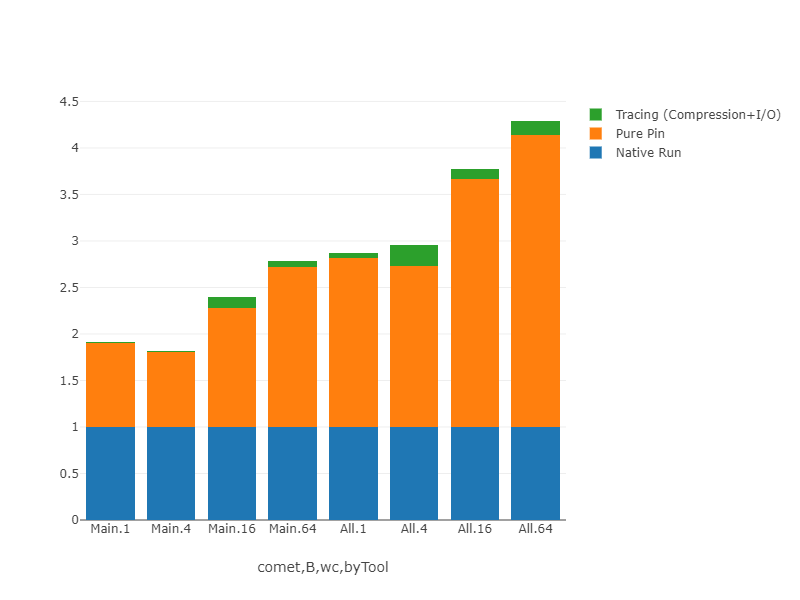
\includegraphics[width=6in]{figs.comet/comet_chartDet_B_wc_byTool_p3_5.png}
\caption{ Input: \textbf{B}
}
\label{comet_chartDet_B_wc_byTool_p3_5}
\end{figure*}


%Figure c wc
\begin{figure*}[!t]
\centering
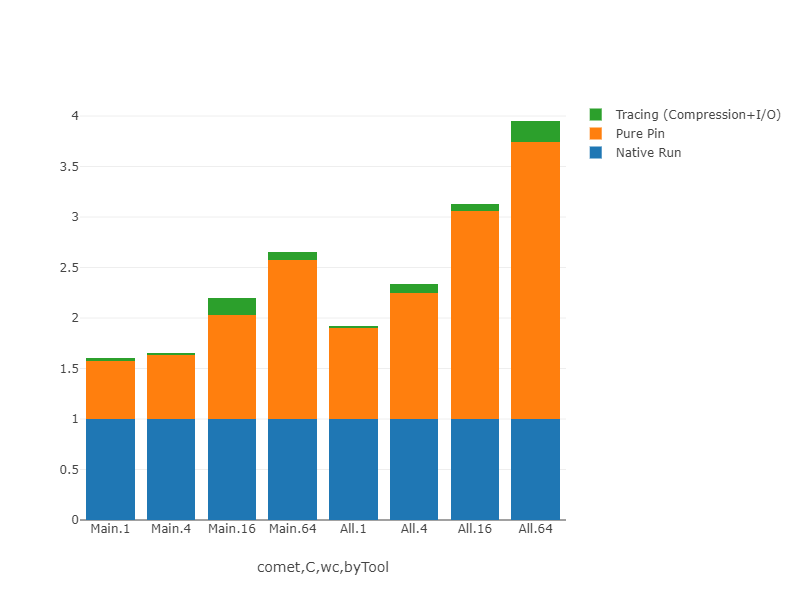
\includegraphics[width=6in]{figs.comet/comet_chartDet_C_wc_byTool_p3_5.png}
\caption{ Input: \textbf{C}
}
\label{comet_chartDet_C_wc_byTool_p3_5}
\end{figure*}





\begin{figure*}[!t]
\centering
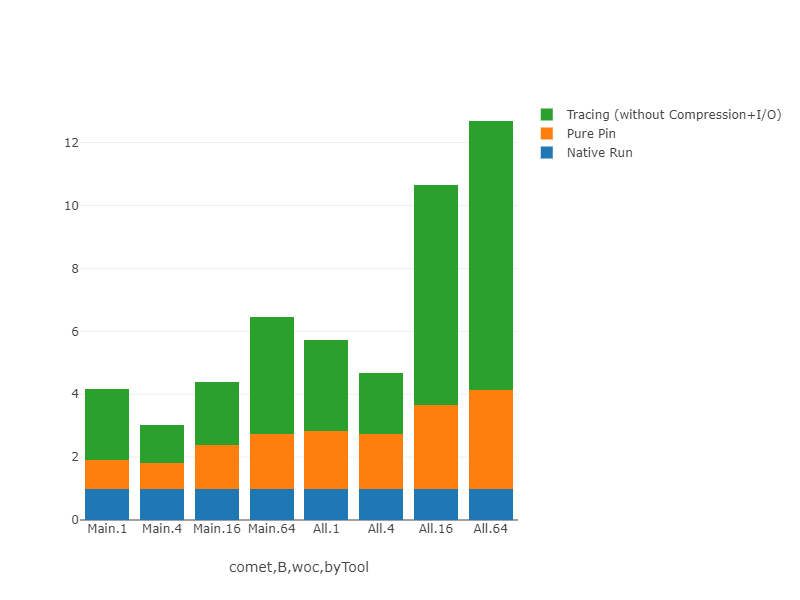
\includegraphics[width=6in]{figs.comet/comet_chartDet_B_woc_byTool_p3_5.png}
\caption{ Input: \textbf{B}
}
\label{comet_chartDet_B_woc_byTool_p3_5}
\end{figure*}

\begin{figure*}[!t]
\centering
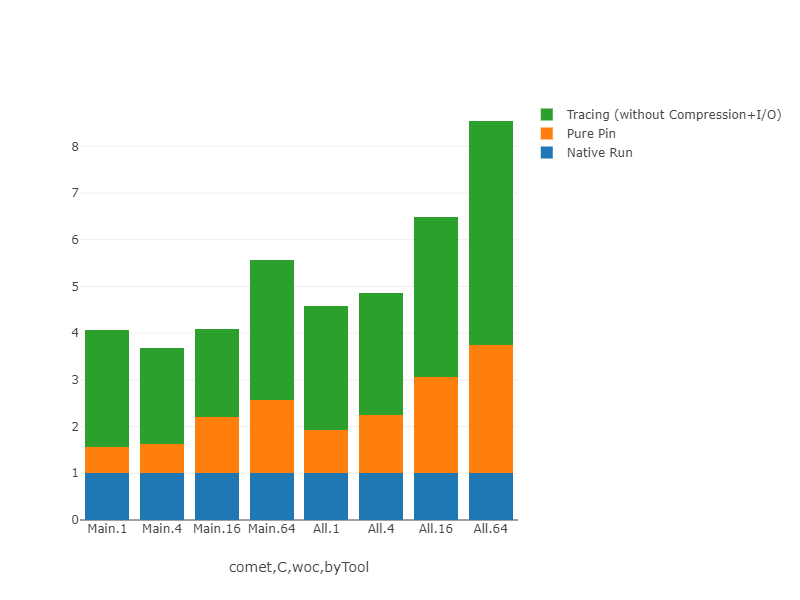
\includegraphics[width=6in]{figs.comet/comet_chartDet_C_woc_byTool_p3_5.png}
\caption{ Input: \textbf{C}
}
\label{comet_chartDet_C_woc_byTool_p3_5}
\end{figure*}







\begin{figure*}[!t]
\centering
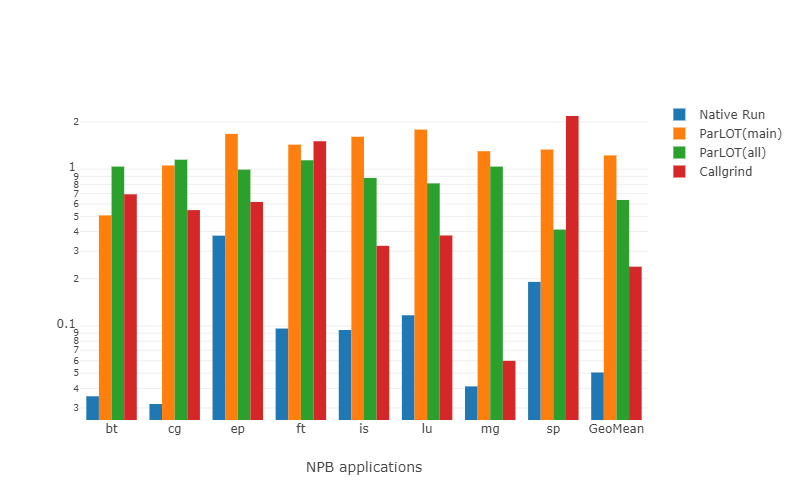
\includegraphics[width=6in]{figs.comet/comet_chartAvg_var_C_p3_5.png}
\caption{ Input: \textbf{C}  - Variance of 3 Runtimes
}
\label{comet_chartAvg_var_C_p3_5}
\end{figure*}



\begin{figure*}[!t]
\centering
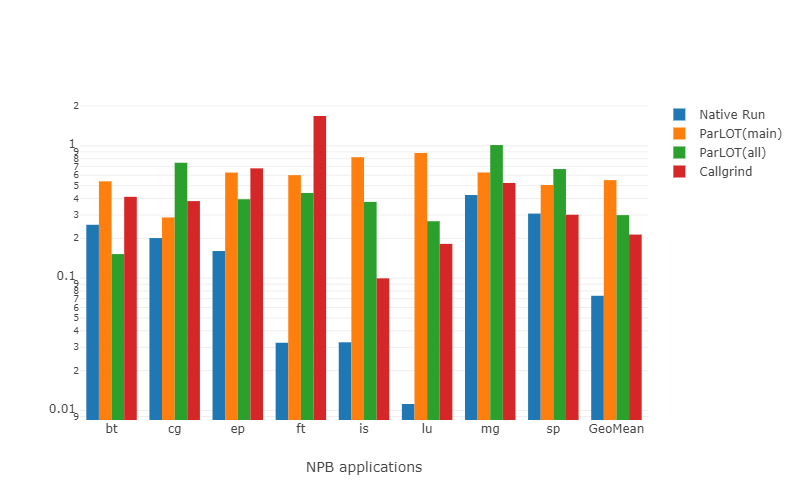
\includegraphics[width=6in]{figs.comet/comet_chartAvg_var_B_p3_5.png}
\caption{ Input: \textbf{B}  - Variance of 3 Runtimes
}
\label{comet_chartAvg_var_B_p3_5}
\end{figure*}









\begin{figure*}[!t]
\centering
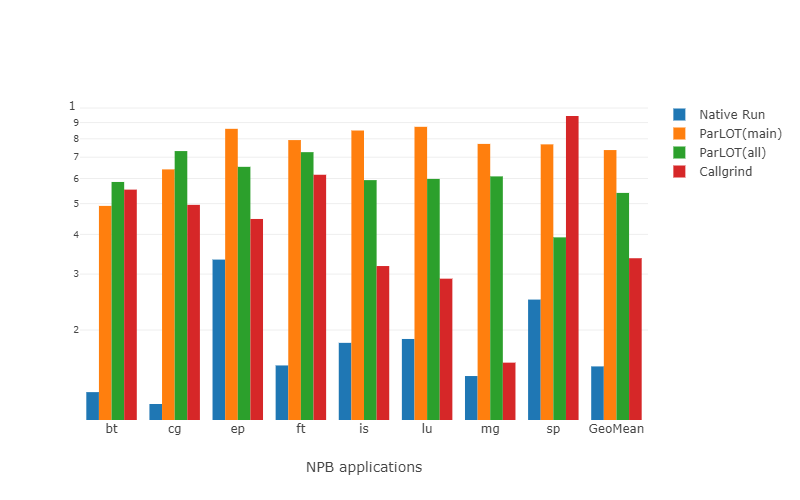
\includegraphics[width=6in]{figs.comet/comet_chartAvg_serr_C_p3_5.png}
\caption{ Input: \textbf{C}  - Standard Error of 3 Runtimes
}
\label{comet_chartAvg_serr_C_p3_5}
\end{figure*}



\begin{figure*}[!t]
\centering
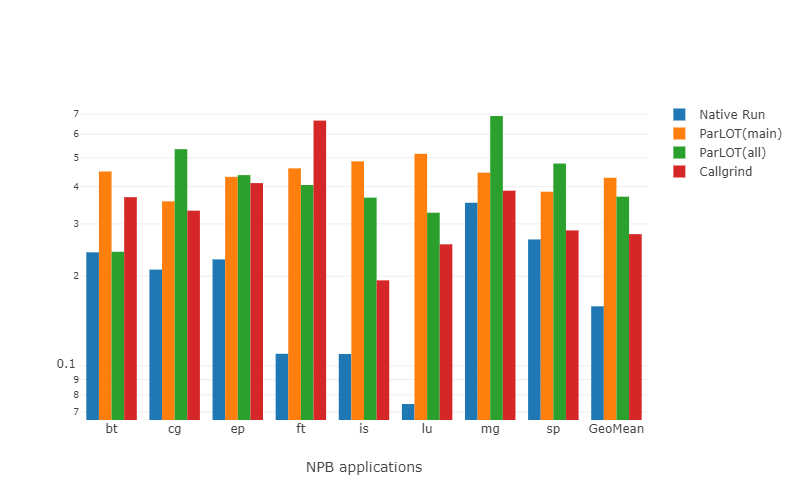
\includegraphics[width=6in]{figs.comet/comet_chartAvg_serr_B_p3_5.png}
\caption{ Input: \textbf{B}  - Standard Error of 3 Runtimes
}
\label{comet_chartAvg_serr_B_p3_5}
\end{figure*}



